%===============================================================================
\section{Norma $H_{\infty}$}
\label{sec:normHinf}

Para o sistema apresentado em (\ref{eq:robust_sis_incert}) a norma $L_2$ deste sistema
� definido como em (\ref{eq:normhinf_l2}).

\begin{equation}
\underset{\left \| \omega(t) \right \|_2 \neq 0}{sup}=\frac{\left \| z(t) \right \|_2}{\left \| \omega(t) \right \|_2}
\label{eq:normhinf_l2}
\end{equation}

Onde a norma $L_2$ de um sinal $\omega(t)$ � definida como abaixo:

\begin{equation}
\left \| \omega(t) \right \|_2 \equiv \sqrt{\int_{0}^{\infty}\omega(t)'w(t) dt}
\nonumber
\end{equation}

Suponha que exista uma fun��o quadr�tica positiva $V(x)=x'Px$ com $P=P'>0$ e um escalar positivo
$\gamma_{\infty}$ tal que:


\begin{equation}
\dot{V}z(t)'z(t)-\gamma_{\infty}^{\omega}\omega(t)'\omega(t)\leq 0
\nonumber
\end{equation}
%===============================================================================
\subsection{Sistemas Lineares sem incertezas}
\label{sec:hinf_sis_lin_sem_incertezas}

Considerando o sistema apresentado em (\ref{eq:robust_sis_incert}) em malha fechada, com 
condi��o inicial nula ($x(0)\equiv 0$) e com $ \Delta (t) \equiv 0$, obt�m-se desta forma
o sistema apresentado em (\ref{eq:sis_mf_incerteza}).

\begin{equation}
\begin{cases}
\dot{x}(t)=(A_0-B_0K)x(t)+B_{\omega}\omega(t)\\ 
z(t)=(G-HK)x(t)
\end{cases}
\label{eq:sis_mf_incerteza}
\end{equation}

A LMI que deve ser satisfeita para que a condi��o de $H_{\infty}$ seja obtida � apresentada
em (\ref{eq:hinf_sem_incerteza}).

\begin{equation}
\begin{matrix}
\begin{bmatrix}
Y & -(GW-HR)'\\ 
 -(GW-HR) & \gamma_{\infty}^2 I  
\end{bmatrix}\geq 0
\\ \\
Y= -WA_0'+R'B_0'-A_0W-B_0R-B_{\omega}B_{\omega}'
\end{matrix}
\label{eq:hinf_sem_incerteza}
\end{equation}

Assim pode-se garantir o limite superior minimo para o ganho $L_2$ do sistema 
(\ref{eq:sis_mf_incerteza}).

Para o caso de sistemas lineares invariantes no tempo a otimiza��o d� exatamente o valor do
ganho $L_2$ que � igual a norma $H_{\infty}$. 

\begin{equation}
T(s)=(G-HK)(sI-(A_0-B_0K))^{-1}B_{\omega}
\nonumber
\end{equation}

Que � equivalente a:

\begin{equation}
\left \| T(s) \right \|_{\infty} \equiv \underset{\omega \in \Re}{max}\sqrt{\lambda (T'(j\omega)T(j\omega))}
\nonumber
\end{equation}

%===============================================================================
\subsection{Incertezas do tipo polit�pico}
\label{sec:hinf_sis_politopico}

No caso de incertezas do tipo polit�picas o limite superior minimo para o ganho $L_2$ pode ser
definido pela equa��o (\ref{eq:hinf_sis_politopico}).

\begin{equation}
\begin{matrix}
\begin{bmatrix}
Y & -(GW-HR)'\\ 
-(GW-HR) & \gamma_{\infty}^2
\end{bmatrix}\geq 0
\\ 
\\ 
Y=-WA_i'+R'B_j'-A_iW+B_jR-B_{\omega}B_{\omega}'
\\ \\
W>0
\end{matrix}
\label{eq:hinf_sis_politopico}
\end{equation}


%===============================================================================
\subsection{Incertezas limitadas em norma}
\label{sec:hinf_sis_norm_limit}

Considerando o sistema descrito em (\ref{eq:robust_sis_incert}) com $\left \| \Delta(t) \right \|\leq 1$.
A condi��o descrita em (\ref{eq:hinf_sem_incerteza}) � equivalente a (\ref{eq:hinf_sis_norm_lim}).

\begin{equation}
\begin{matrix}
\begin{bmatrix}
Y &(E_AW-E_BR)' & -(GW-HR)'\\ 
(E_AW-E_BR) & I & 0\\
-(GW-HR) & 0& \gamma_{\infty}^2
\end{bmatrix}\geq 0
\\ 
\\ 
Y=-WA_0'+R'B_0'-A_0W+B_0R-B_{\omega}B_{\omega}'
\\ \\
W>0
\end{matrix}
\label{eq:hinf_sis_norm_lim}
\end{equation}

Satisfazendo a equa��o (\ref{eq:hinf_sis_norm_lim}) obt�m-se o limite superior minimo para o
ganho $L_2$ e se o sistema for linear e invariante no tempo este valor ser� o mesmo da norma 
$H_{\infty}$ da fun��o de transfer�ncia entre $\omega$ e $z$.

%===============================================================================
\subsubsection{Simula��o}

A resolu��o do sistema de LMIs (\ref{eq:hinf_sis_norm_lim}) gerou os seguintes resultados:

\begin{equation}
\begin{matrix}
W=\begin{bmatrix}
0.2449 & -0.0315\\
-0.0315 &   0.8360
\end{bmatrix}\\ \\ 
R=1.10^3\begin{bmatrix}
 0.0010 & -7.8417
\end{bmatrix}
\\ \\
K=1.10^3\begin{bmatrix}
-1.2096 &  -9.4257
\end{bmatrix}
\\ \\
\gamma_{\infty}^2 = 0.07
\\
\lambda_1=-0.0529\\
\lambda_2=-1.6550
\end{matrix}
\nonumber
\end{equation}

A simula��o do sistema em malha fechada com o ganho $K$ encontrado obtem a resposta
apresentada na Figura (\ref{fig:hinf_norm_bounded}). Os valores de $\lambda_1$ e $\lambda_2$ 
s�o os autovalores do sistema em malha fechada.

\begin{figure}[htbp]
	\center
	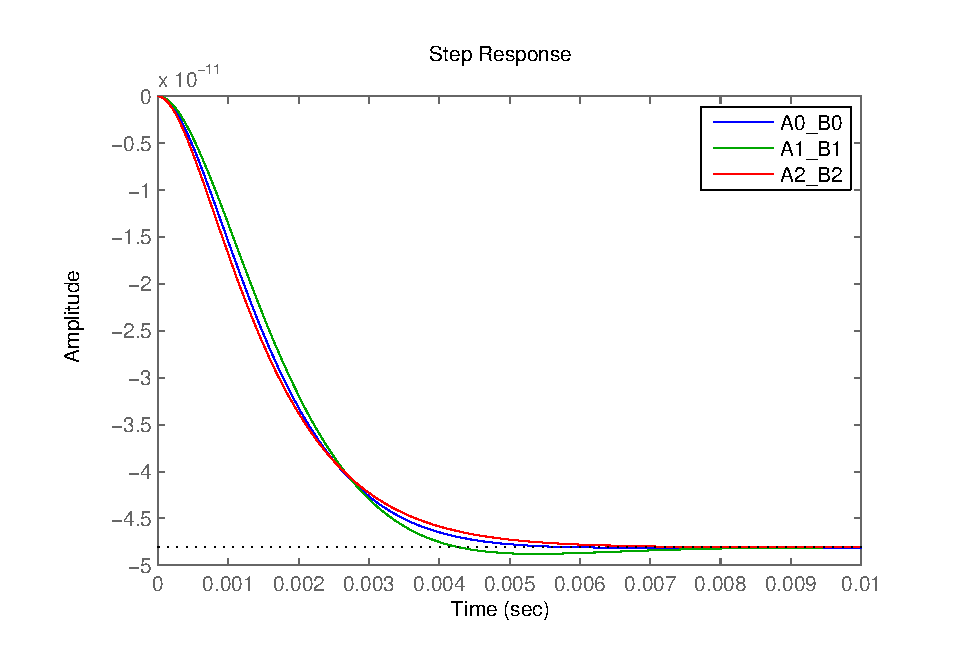
\includegraphics[width=0.95\columnwidth]{figures/hinf_norm_bounded.eps}
	\caption{Resposta do sistema (\ref{eq:sis_mf_incerteza}) com o ganho K encontrado 
		pelo crit�rio de $H_{\infty}$}
	\label{fig:hinf_norm_bounded}
\end{figure}


%===============================================================================
